
The domain is a unit square. Fluids are such that 
$\rho_1=1$, $\eta_1=1$ and $\rho_2=1.01$, $\eta_2=1000$.
Boundary conditions are either free slip or no slip on all sides. 
Pressure is normalised so that the volume average is zero. 
Gravity points downwards with $|\vec{g}|=1$.
Profile measurements are carried out on the dashed line.


\begin{center}
\begin{tikzpicture}
%\draw[fill=gray!23,gray!23](0,0) rectangle (6,4.5);
\draw[step=0.5cm,gray,very thin] (0,0) grid (6,5); %background grid

\fill[green!10!white] (0.5,0.5) -- (4.5,0.5) -- (4.5,4.5) --  (0.5,4.5) --cycle ; 
\draw[line width=0.5mm] (0.5,0.5) -- (4.5,0.5) -- (4.5,4.5) --  (0.5,4.5) --cycle ; 

\fill[blue!40!white] (2.25,2.25) -- (2.75,2.25) -- (2.75,2.75) --  (2.25,2.75) --cycle ; 
\draw[thick] (2.25,2.25) -- (2.75,2.25) -- (2.75,2.75) --  (2.25,2.75) --cycle ; 

\draw [->] (5.,3) -- (5.,2);
\node[] at (5.25,2.5) {$\vec{g}$};

\node[] at (1.5,1.5) {$\rho_1,\eta_1$};
\node[] at (2.47,2.95) {$\rho_2,\eta_2$};

\draw[thick, >=triangle 45, ->] (4.5,0.5) -- (5,0.5);
\draw[thick, >=triangle 45, ->] (0.5,4.5) -- (0.5,5);

\node[] at (4.7,0.2) {$x$};
\node[] at (0.2,4.7) {$y$};

\draw[dashed] (2.5,0.5) -- (2.5,4.5);

\end{tikzpicture}


\end{center}

When using \aspect{}, it is good to remember that a compositional field is used, 
which 'lives' on the nodes of the FE grid. Partof the input file is shown here: 

\begin{verbatim}
subsection Compositional fields
  set Number of fields = 1 
end 

subsection Initial composition model
  set Model name = function
  subsection Function
    set Variable names      = x,y 
    set Function constants  = p=0.5
    set Function expression = if(abs(x-p)<0.0625 && abs(y-p)<0.0625 , 1, 0)
  end 
end

subsection Material model
  subsection Simple model
    set Density differential for compositional field 1 = 0.01
    set Composition viscosity prefactor = 1000
  end 
end
\end{verbatim}

The value of the composition (and therefore 
the density and viscosity values) on a quadrature point is obtained via interpolation 
and averaging, which is different than the Stone codes where the density 
and viscosity are elemental quantities.

\newpage
%...................................................................
\paragraph{Free-slip boundary conditions}.

\begin{center}
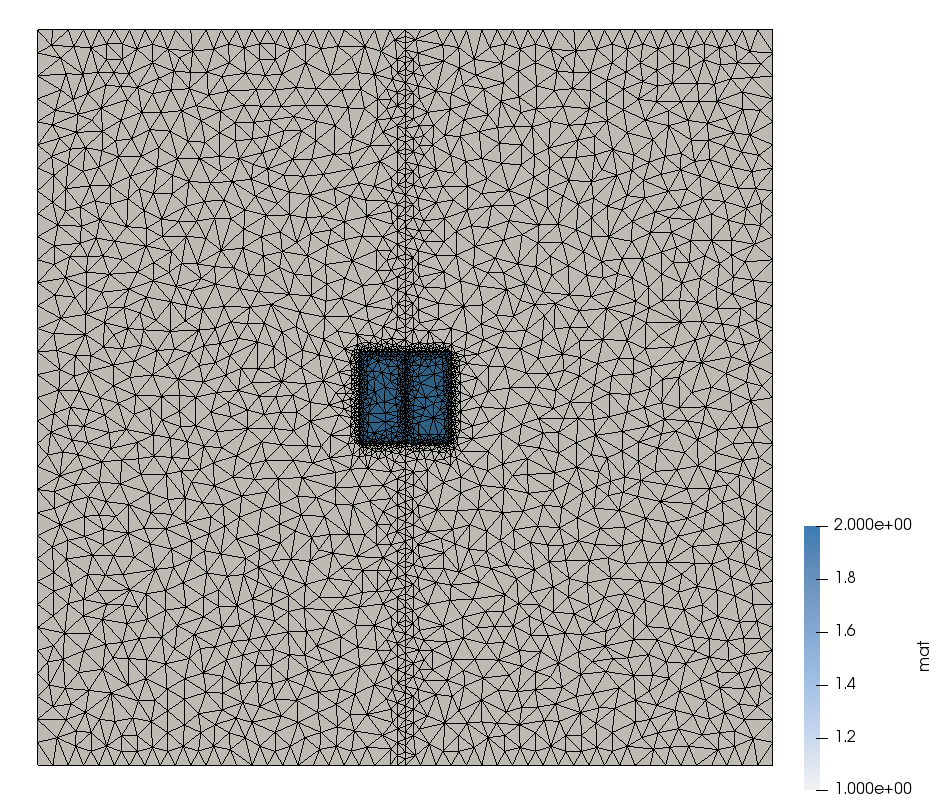
\includegraphics[width=5.cm]{images/sinking_block/FS/stone93/grid}
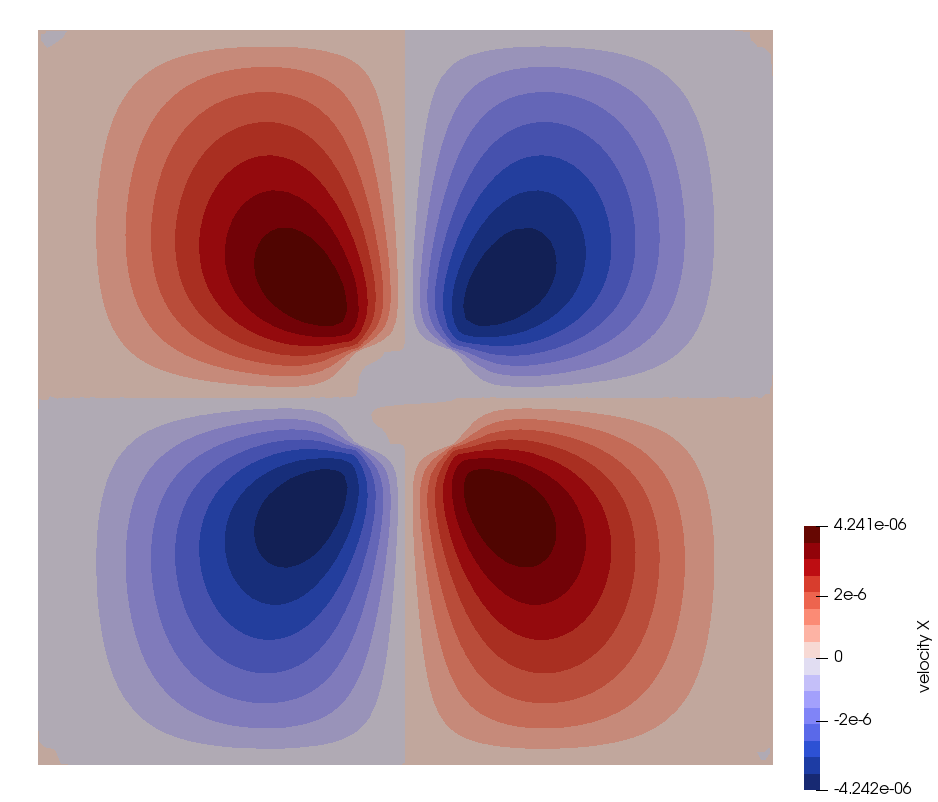
\includegraphics[width=5.cm]{images/sinking_block/FS/stone93/u}
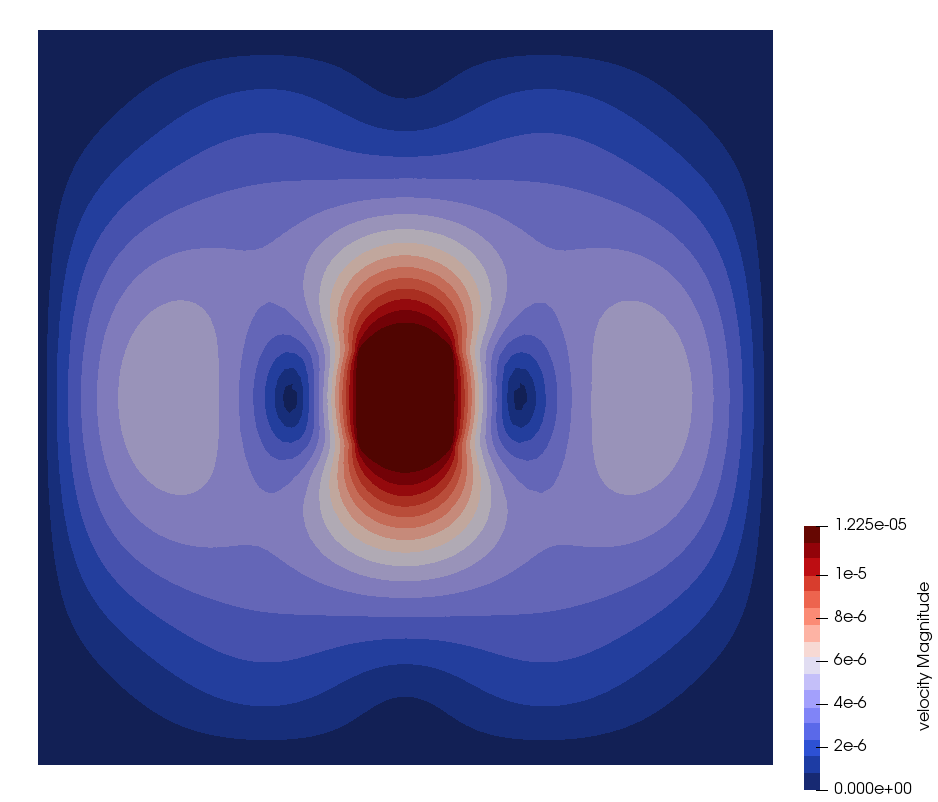
\includegraphics[width=5.cm]{images/sinking_block/FS/stone93/vel}\\
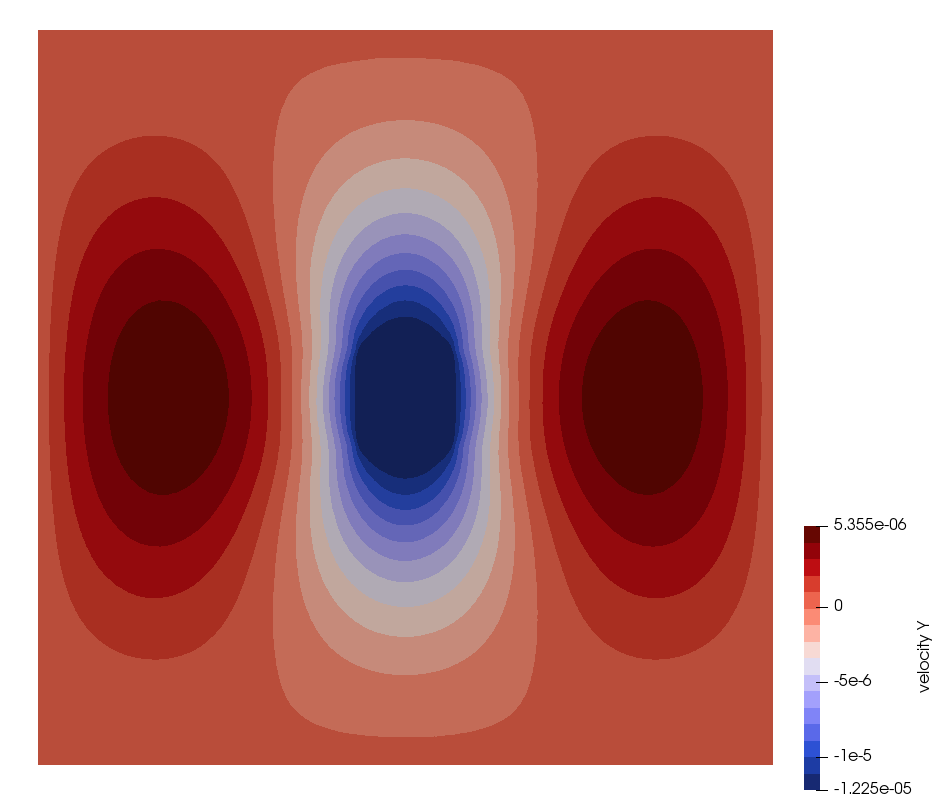
\includegraphics[width=5.cm]{images/sinking_block/FS/stone93/v}
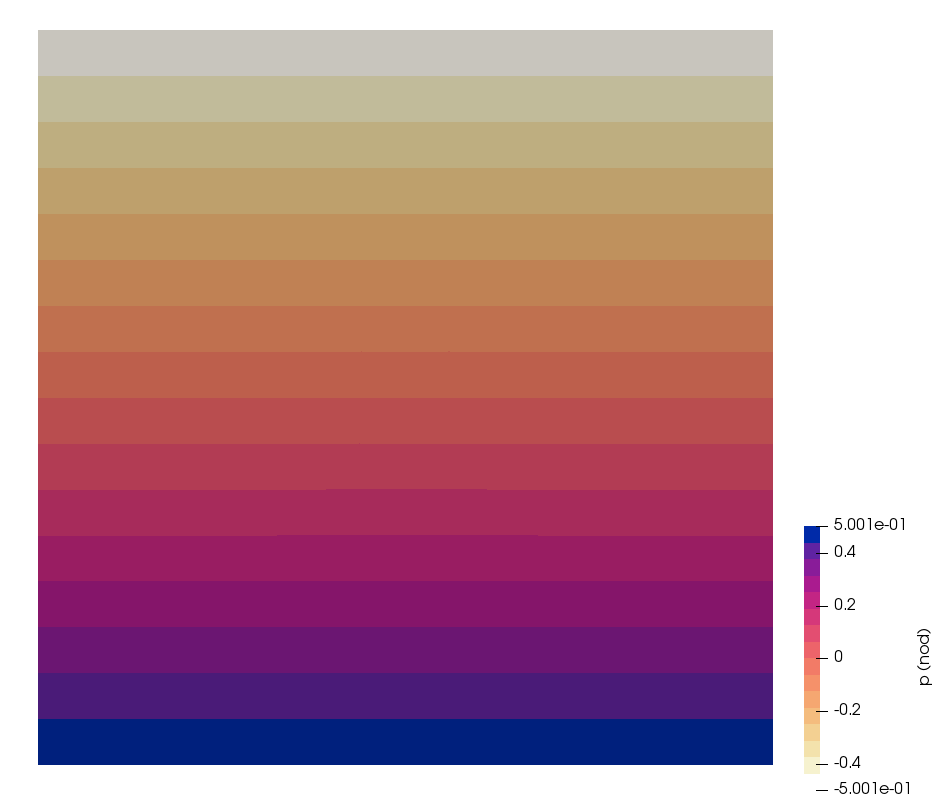
\includegraphics[width=5.cm]{images/sinking_block/FS/stone93/press}
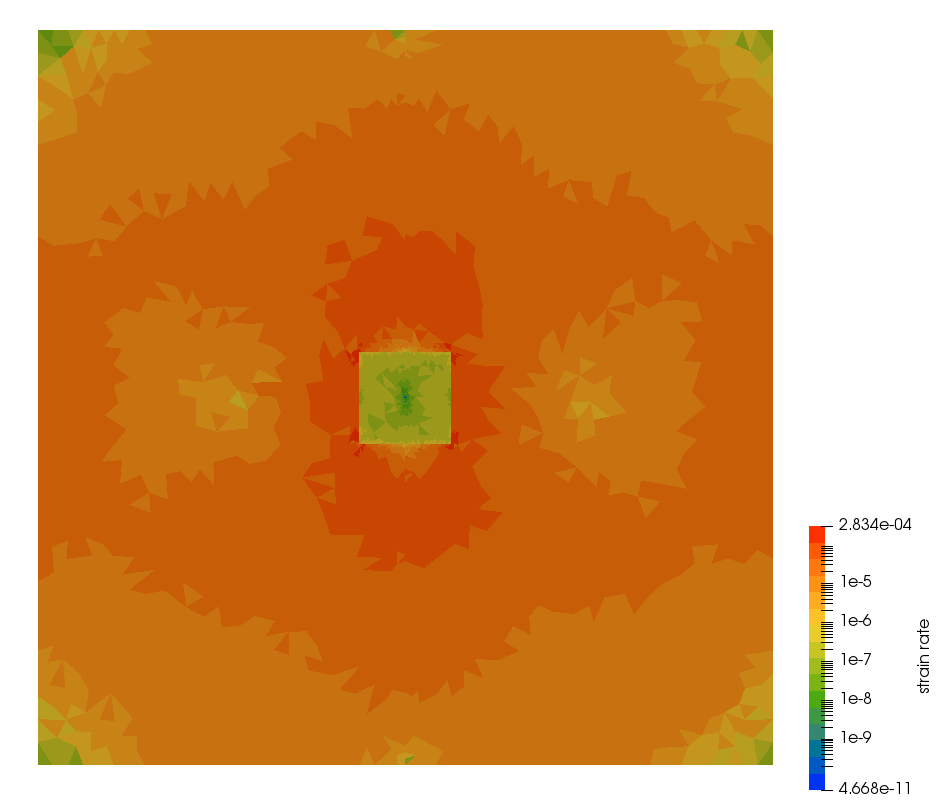
\includegraphics[width=5.cm]{images/sinking_block/FS/stone93/sr}\\
{\captionfont Results obtained with Stone 93.}
\end{center}

\begin{center}
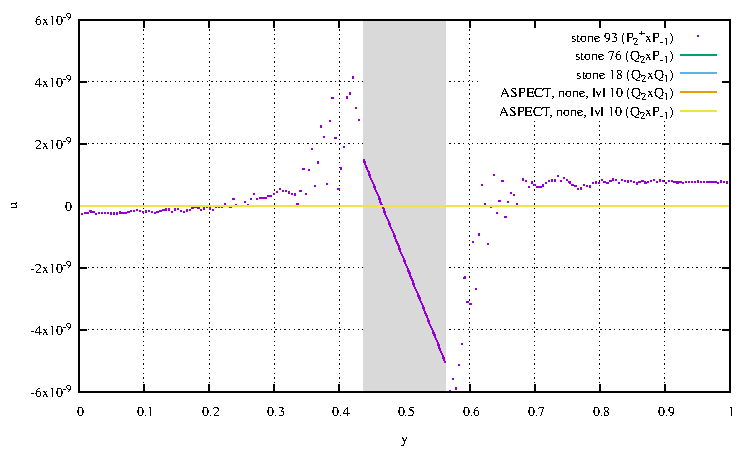
\includegraphics[width=5.6cm]{images/sinking_block/u_FS}
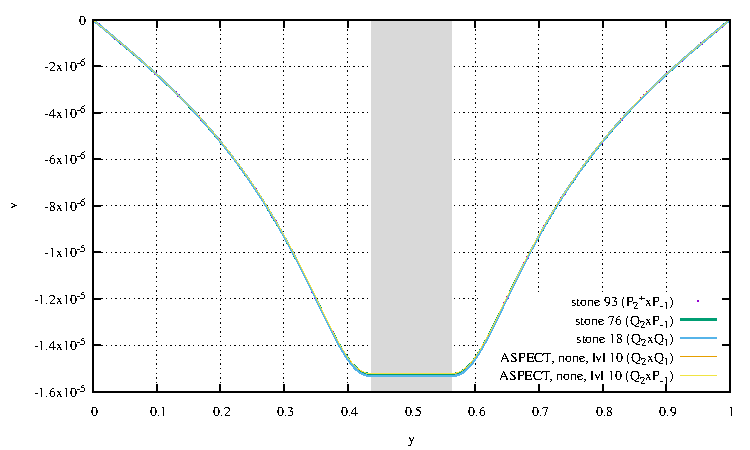
\includegraphics[width=5.6cm]{images/sinking_block/v_FS}
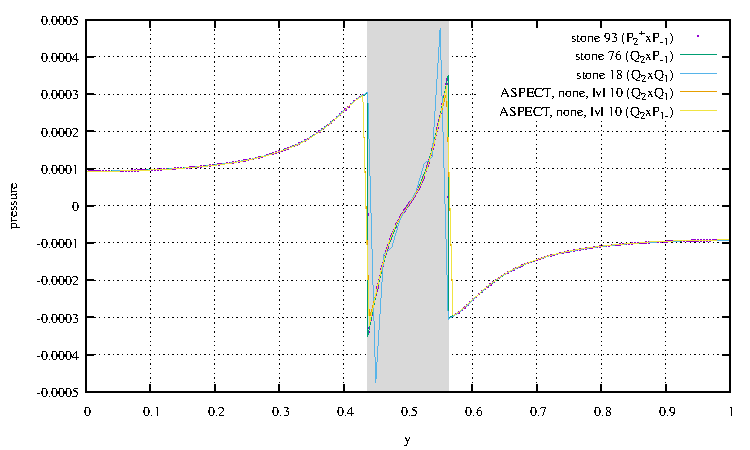
\includegraphics[width=5.6cm]{images/sinking_block/pressure_FS}\\
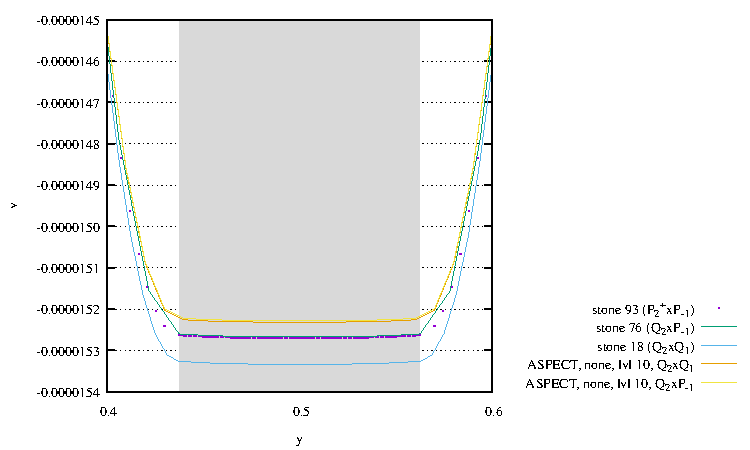
\includegraphics[width=5.6cm]{images/sinking_block/v_FS_zoom}
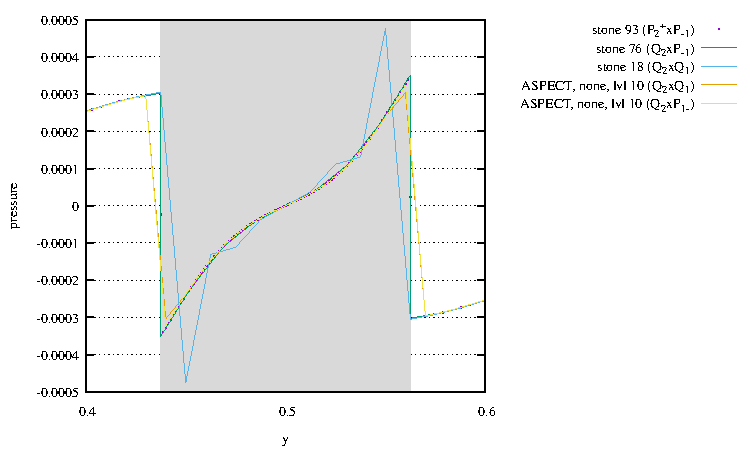
\includegraphics[width=5.6cm]{images/sinking_block/pressure_FS_zoom}\\
\end{center}


\begin{center}
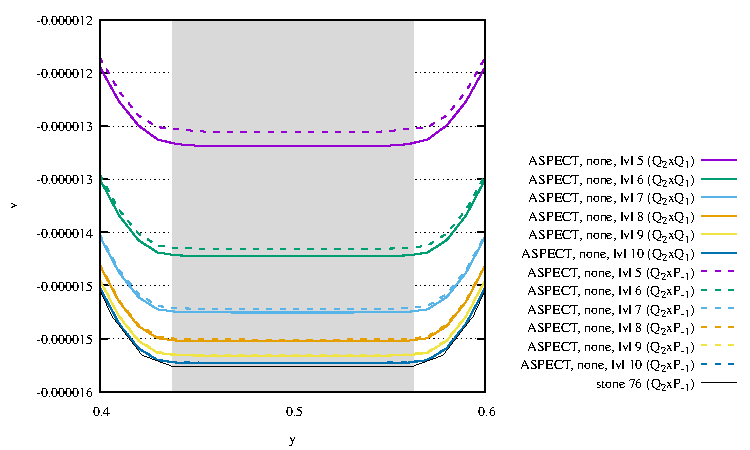
\includegraphics[width=7cm]{images/sinking_block/v_FS_ASPECT_56789}
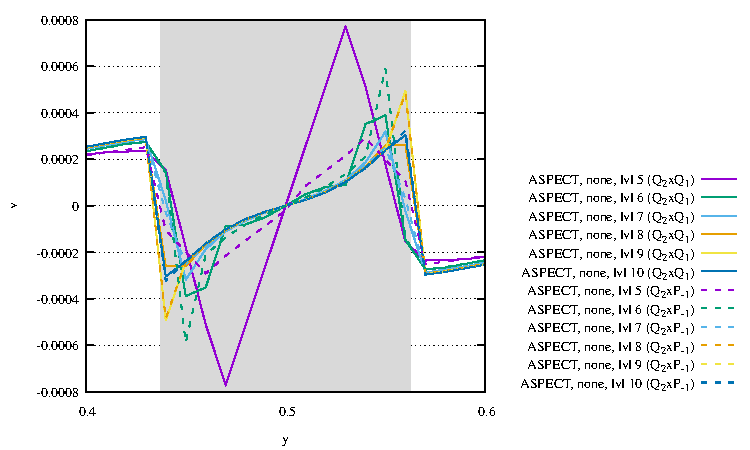
\includegraphics[width=7cm]{images/sinking_block/pressure_FS_ASPECT_56789}\\
{\captionfont ASPECT results with various global mesh refinement. No averaging}
\end{center}

\begin{center}
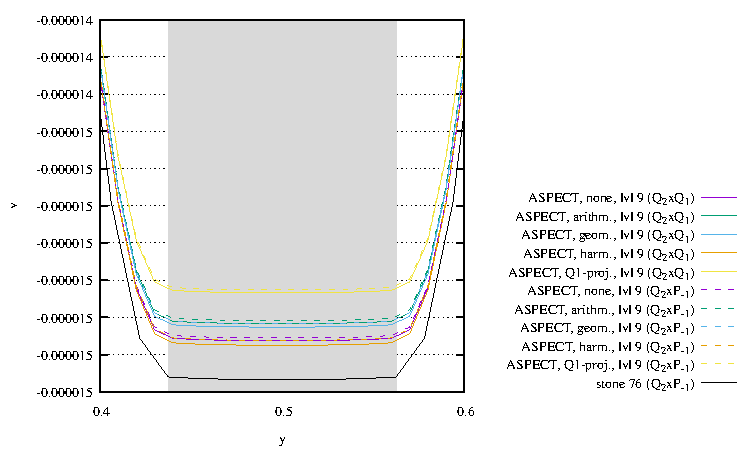
\includegraphics[width=7cm]{images/sinking_block/v_FS_ASPECT_avrg}
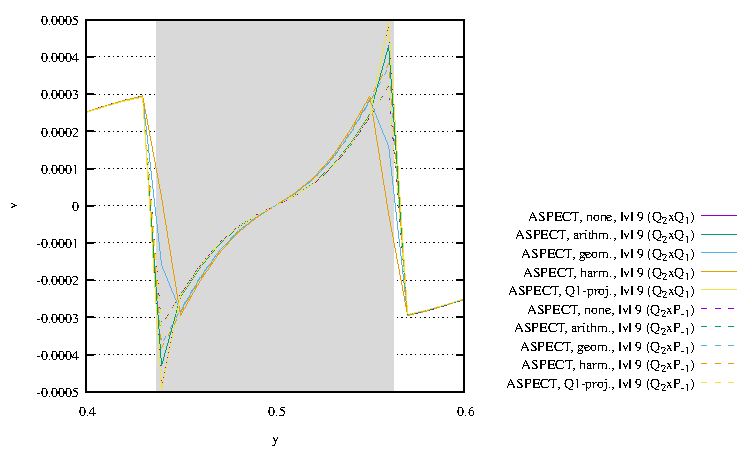
\includegraphics[width=7cm]{images/sinking_block/pressure_FS_ASPECT_avrg}\\
{\captionfont ASPECT results with various averagings. level 9.}
\end{center}



\begin{center}
\begin{tabular}{llp{4cm}p{4cm}}
\hline
            &  & FS & NS \\ 
\hline\hline
$\min(u)$   & Stone 18 ($Q_2\times Q_1$) &  &    \\ 
            & Stone 93 ($P_2^+\times P_{-1}$) &  &   \\
            & Stone 76 ($Q_2\times P_{-1}$) & & \\
            & Aspect   &  &         \\
\hline
$\max(u)$   & Stone 18 ($Q_2\times Q_1$) &  &    \\ 
            & Stone 93 ($P_2^+\times P_{-1}$)&  &         \\
            & Stone 76 ($Q_2\times P_{-1}$) & & \\
            & Aspect   &  &         \\
\hline
$\min(v)$   & Stone 18 ($Q_2\times Q_1$) &  &    \\ 
            & Stone 93 ($P_2^+\times P_{-1}$)&  &         \\
            & Stone 76 ($Q_2\times P_{-1}$) & & \\
            & Aspect   &           \\
\hline
$\max(v)$   & Stone 18 ($Q_2\times Q_1$) &  &    \\ 
            & Stone 93 ($P_2^+\times P_{-1}$)&  &         \\
            & Stone 76 ($Q_2\times P_{-1}$) & & \\
            & Aspect   &   &        \\
\hline
$\max(|v|)$ & Stone 18 ($Q_2\times Q_1$) &  &    \\ 
            & Stone 93 ($P_2^+\times P_{-1}$)&  &         \\
            & Stone 76 ($Q_2\times P_{-1}$) & & \\
            & Aspect   &   &        \\
\hline
$v_{rms}$   & Stone 18 ($Q_2\times Q_1$) &  &    \\ 
            & Stone 93 ($P_2^+\times P_{-1}$)&  &         \\
            & Stone 76 ($Q_2\times P_{-1}$) & & \\
            & Aspect   &          \\
\hline
$\min(p)$   & Stone 18 ($Q_2\times Q_1$) &  &    \\ 
            & Stone 93 ($P_2^+\times P_{-1}$)&  &         \\
            & Stone 76 ($Q_2\times P_{-1}$) & & \\
            & Aspect   &          \\
\hline
$\max(p)$   & Stone 18 ($Q_2\times Q_1$) &  &    \\ 
            & Stone 93 ($P_2^+\times P_{-1}$)&  &         \\
            & Stone 76 ($Q_2\times P_{-1}$) & & \\
            & Aspect   &   &        \\
\hline
$|v|(0.5,0.5)$ & Stone 18 ($Q_2\times Q_1$) &  &    \\ 
            & Stone 93 ($P_2^+\times P_{-1}$)&  &         \\
            & Stone 76 ($Q_2\times P_{-1}$) & & \\
            & Aspect   &   &        \\
\hline
\end{tabular}
\end{center}


Using error extrapolation (see Section~\ref{ss:extrapolation}), one can compute an 
estimate of the resolution independent value of the vrms of maximum velocity for example:

\begin{center}
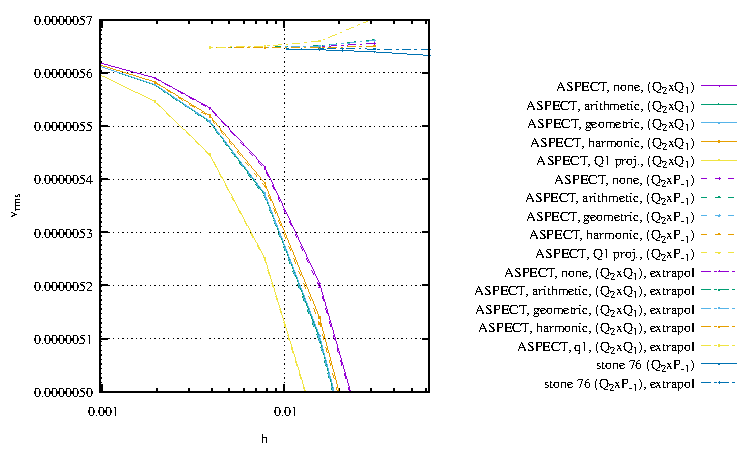
\includegraphics[width=5cm]{images/sinking_block/vrms_FS}
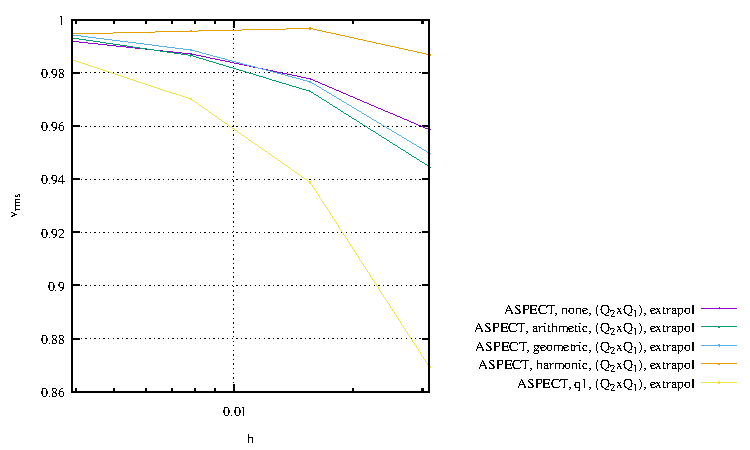
\includegraphics[width=5cm]{images/sinking_block/vrms_FS_extrapolation_rate}
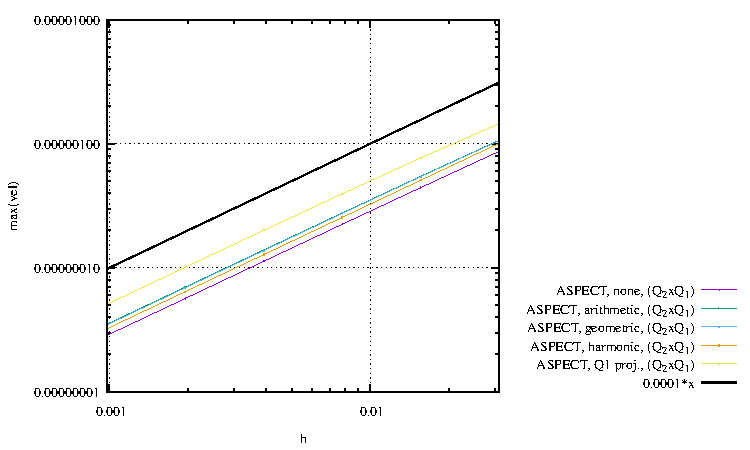
\includegraphics[width=5cm]{images/sinking_block/vrms_FS_error}\\
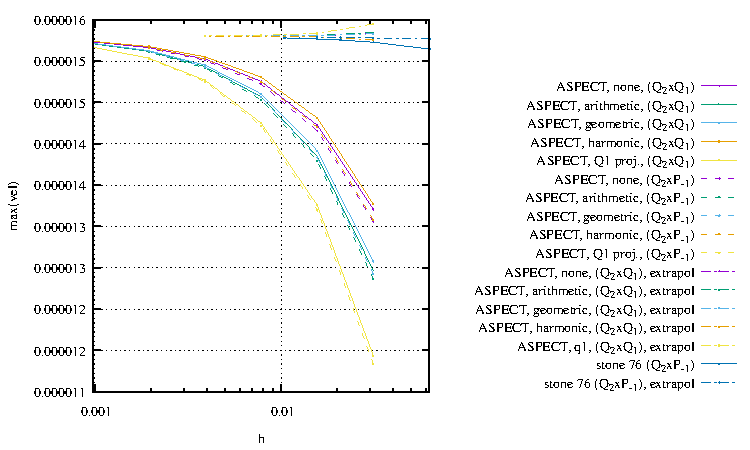
\includegraphics[width=5cm]{images/sinking_block/maxvel_FS}
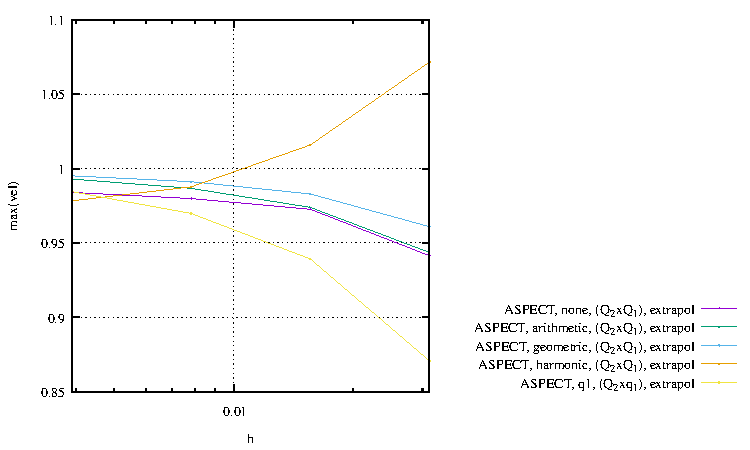
\includegraphics[width=5cm]{images/sinking_block/maxvel_FS_extrapolation_rate}
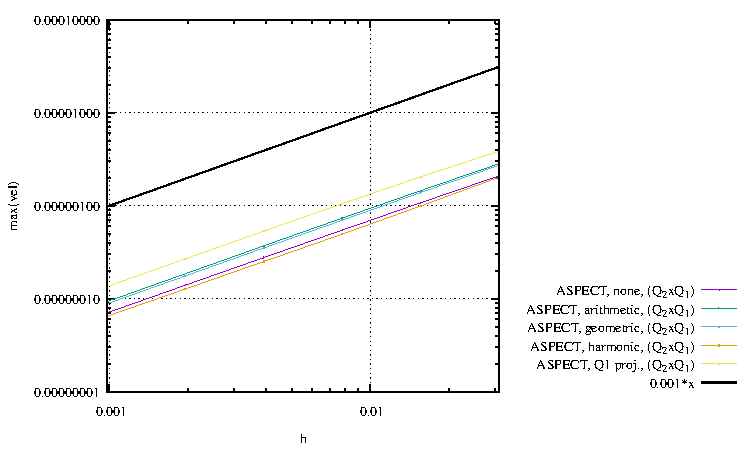
\includegraphics[width=5cm]{images/sinking_block/maxvel_FS_error}
\end{center}

We find that the rates are near unity.


TODO: write material model in ASPECT to bypass compositions! 



\newpage
%......................................................................................
\paragraph{No-slip boundary conditions}.

\begin{center}
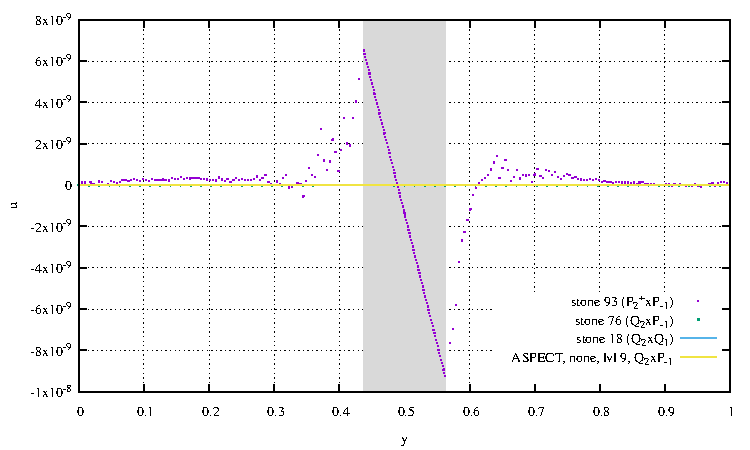
\includegraphics[width=5.6cm]{images/sinking_block/u_NS}
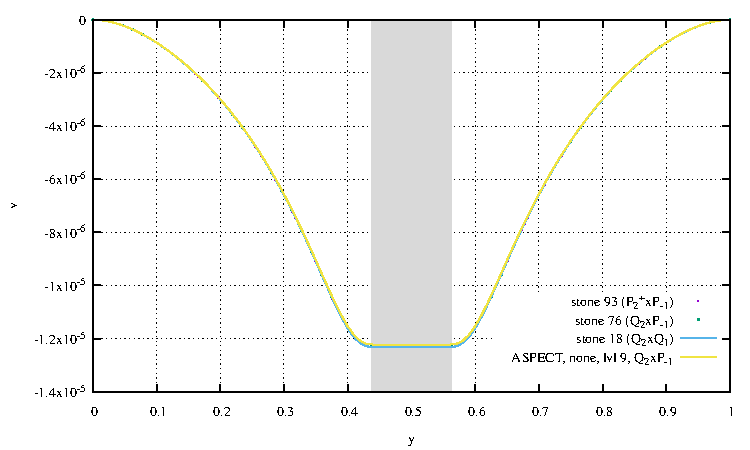
\includegraphics[width=5.6cm]{images/sinking_block/v_NS}
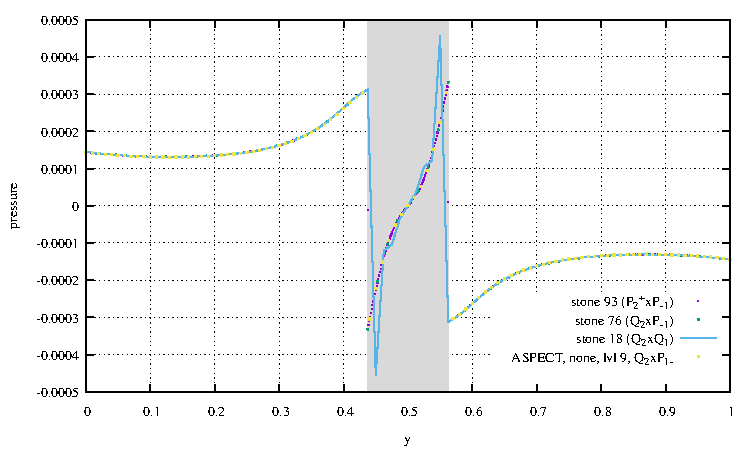
\includegraphics[width=5.6cm]{images/sinking_block/pressure_NS}
\end{center}

\begin{center}
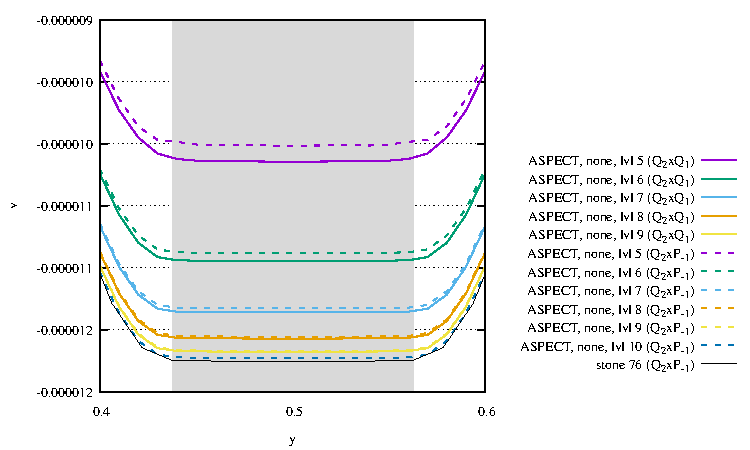
\includegraphics[width=7cm]{images/sinking_block/v_NS_ASPECT_56789}
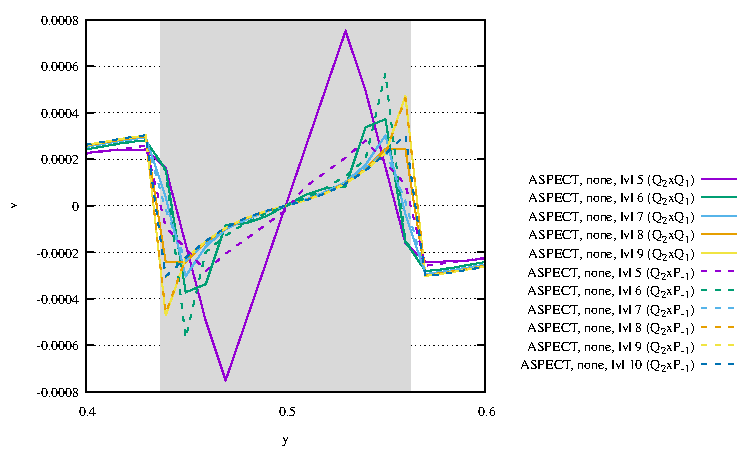
\includegraphics[width=7cm]{images/sinking_block/pressure_NS_ASPECT_56789}\\
{\captionfont ASPECT results with various global mesh refinement. No averaging}
\end{center}

\begin{center}
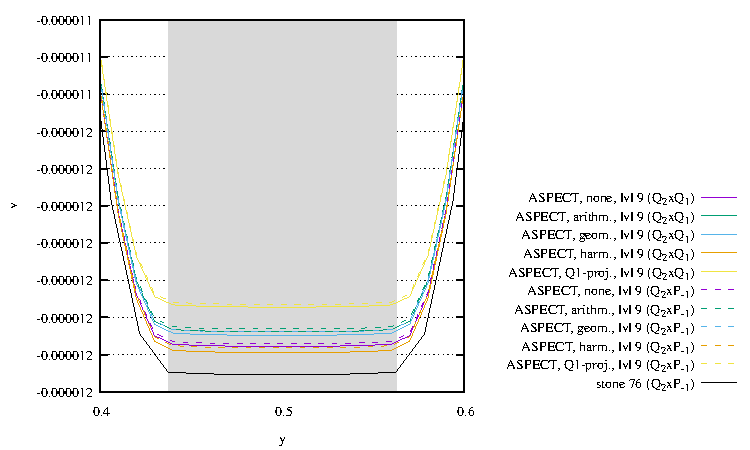
\includegraphics[width=7cm]{images/sinking_block/v_NS_ASPECT_avrg}
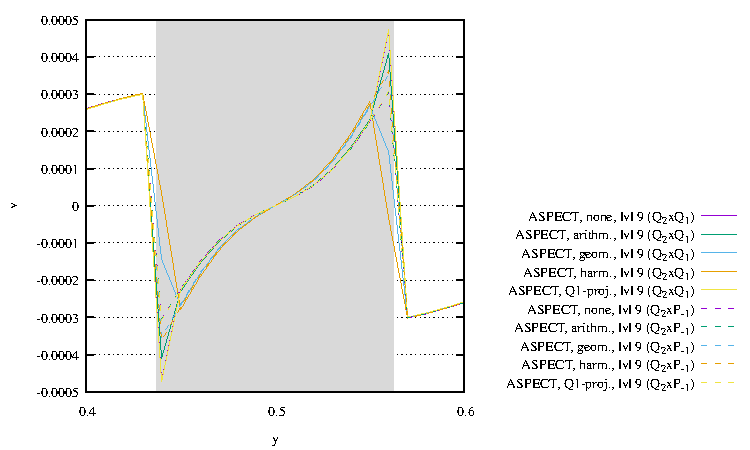
\includegraphics[width=7cm]{images/sinking_block/pressure_NS_ASPECT_avrg}\\
{\captionfont ASPECT results with various averagings. level 9.}
\end{center}


\begin{center}
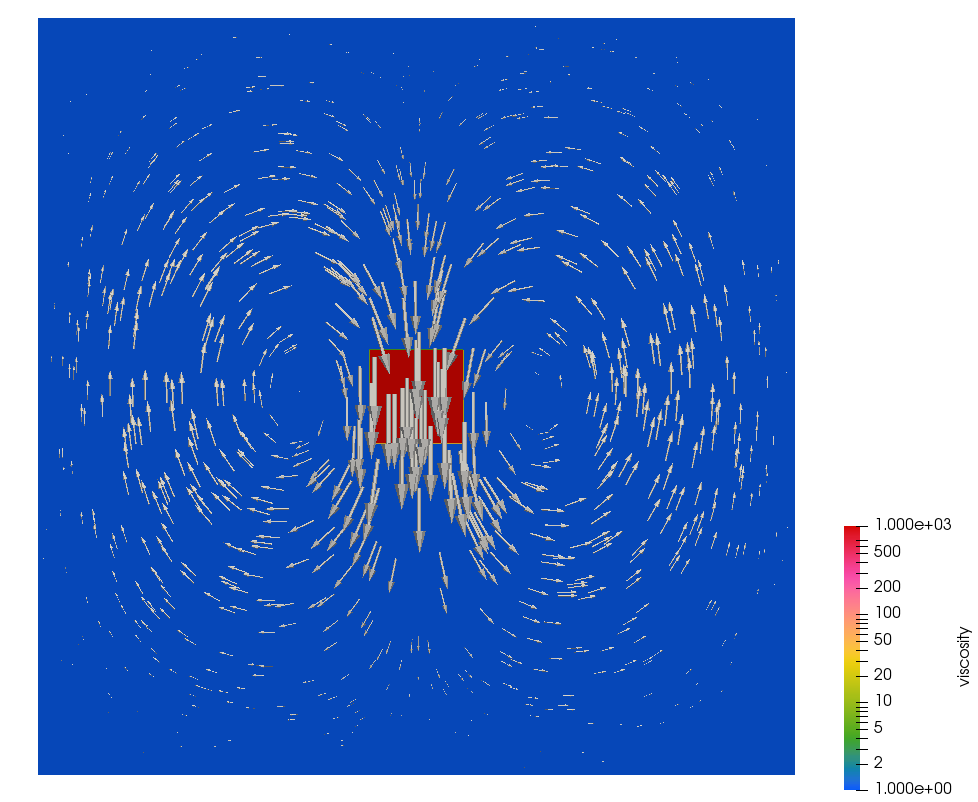
\includegraphics[width=5.7cm]{images/sinking_block/NS/ASPECT/q2q1/eta}
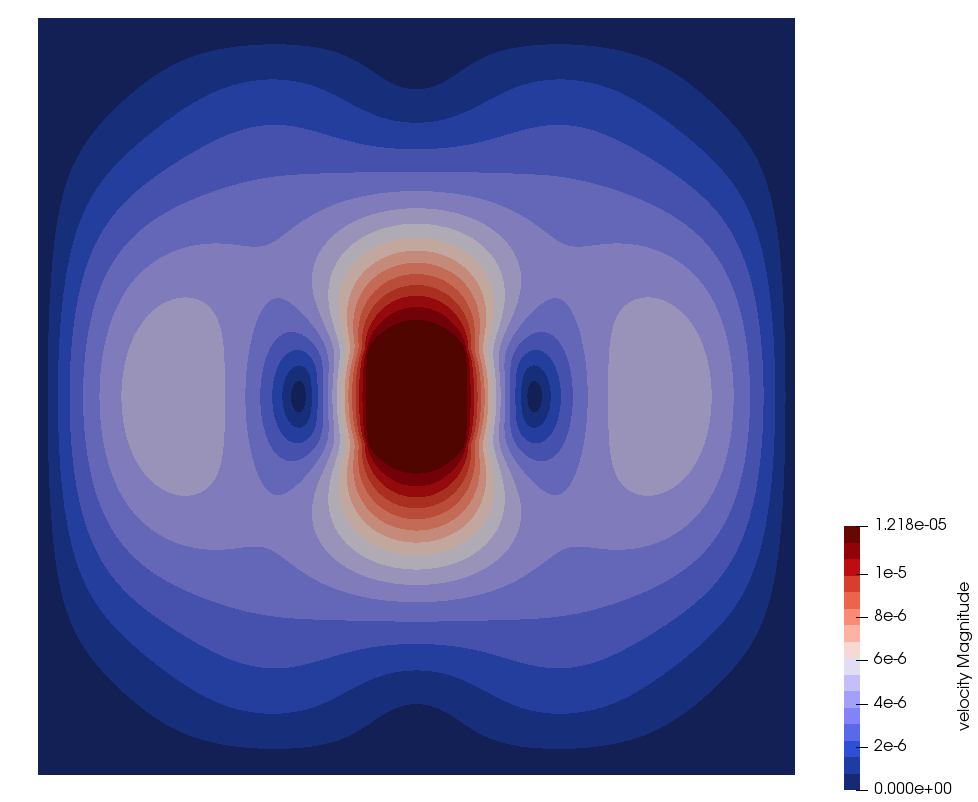
\includegraphics[width=5.7cm]{images/sinking_block/NS/ASPECT/q2q1/vel}
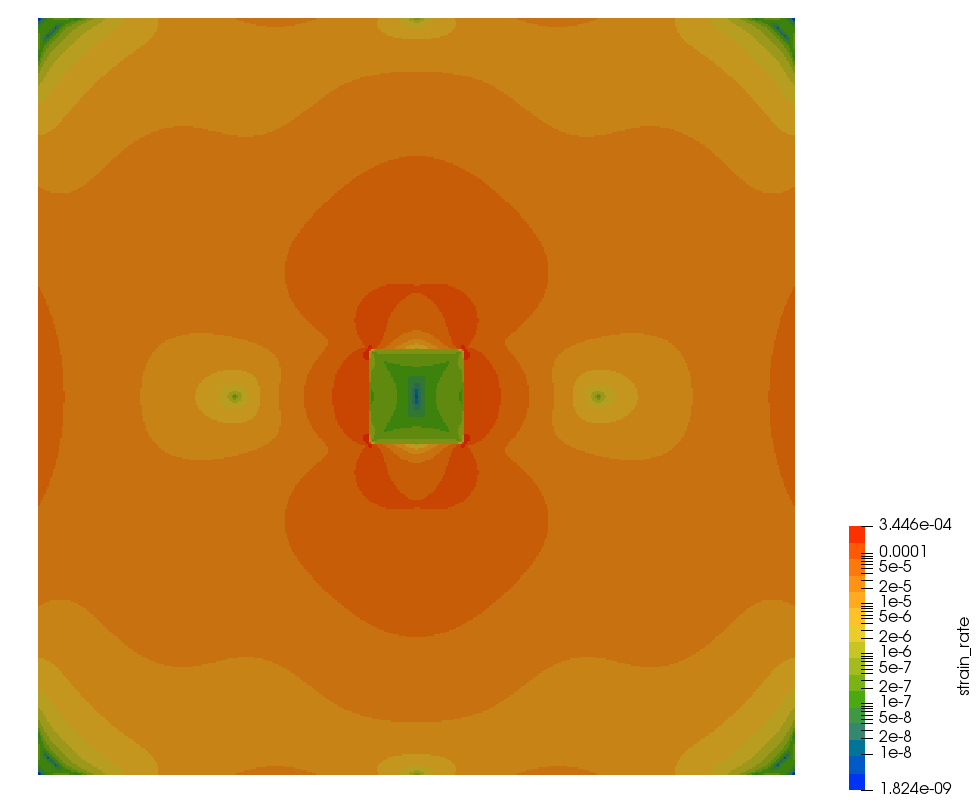
\includegraphics[width=5.7cm]{images/sinking_block/NS/ASPECT/q2q1/sr}\\
{\captionfont Obtained with ASPECT, level 9.}
\end{center}

TODO: finish analysis








